%\nosectionpage
\section{Do-it-yourself-Geräte}
%\withsectionpage

\begin{frame}{LoRaWAN: \alert{Do It Yourself} Gateway}
\begin{columns}
    \begin{column}{0.6\linewidth}
        \begin{center}
            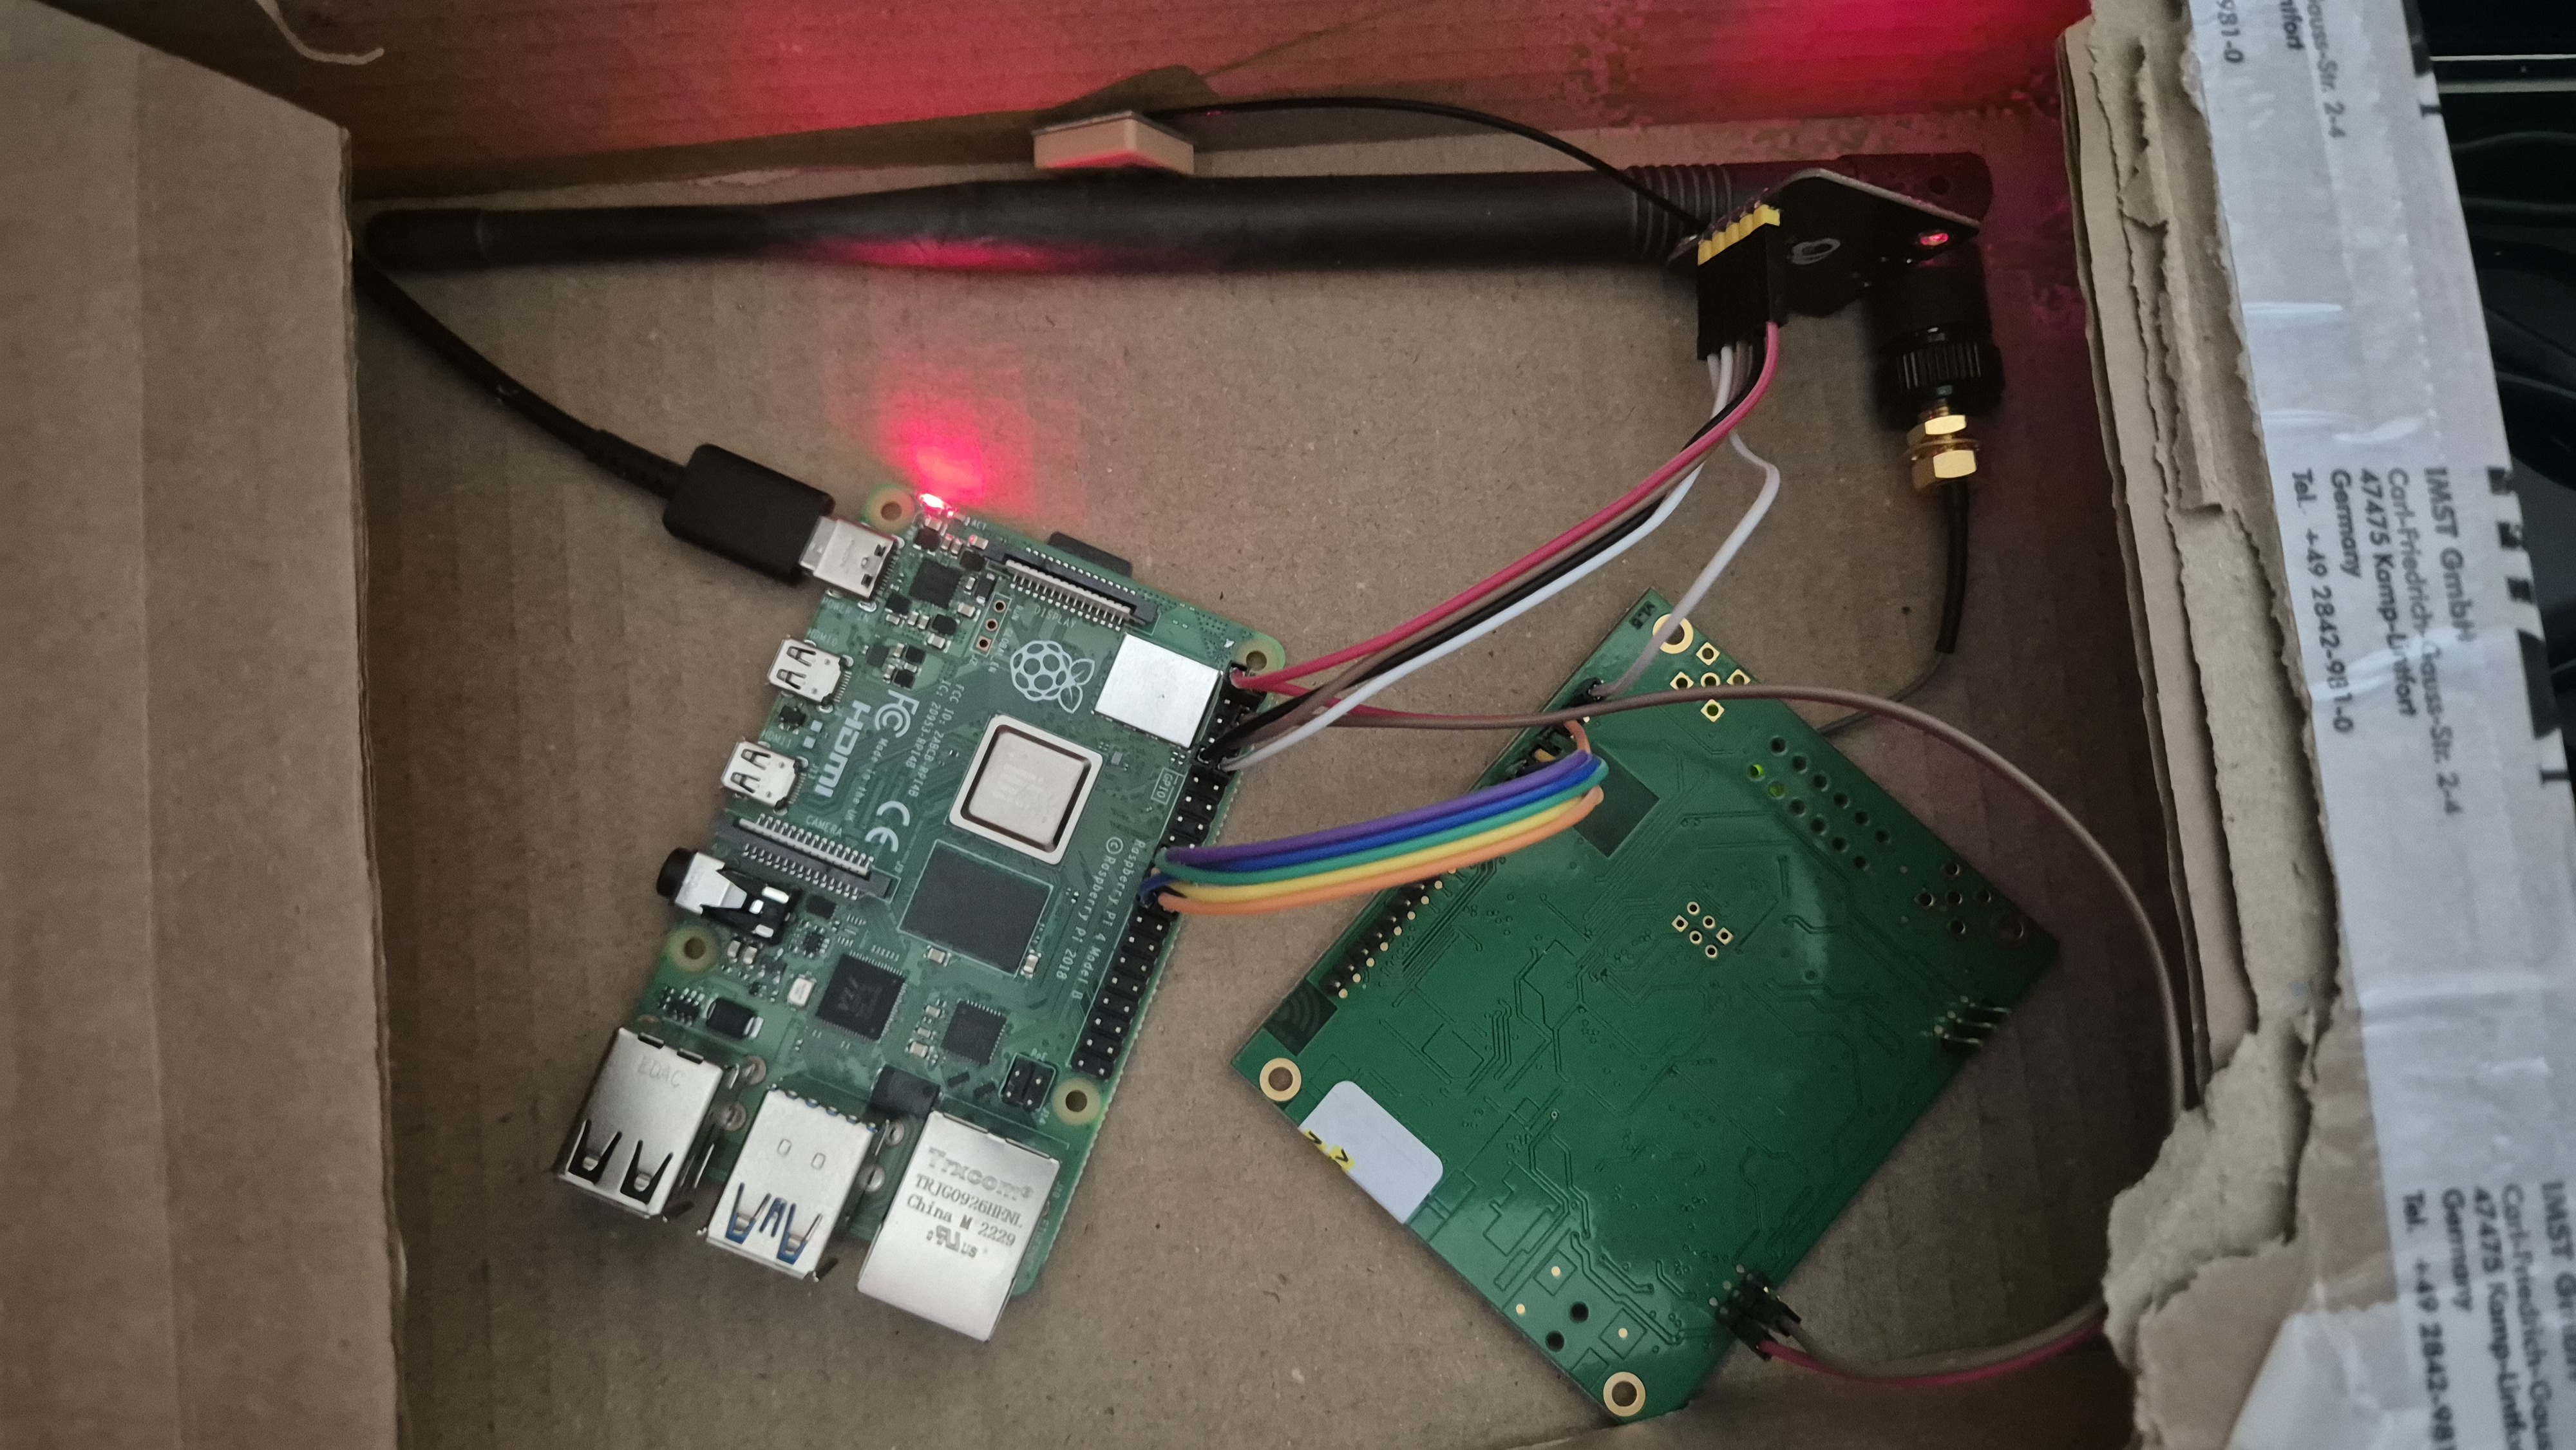
\includegraphics[width=1\textwidth]{material/gateway-prototype.jpg}
        \end{center}
    \end{column}
    \begin{column}{0.4\linewidth}
        \begin{center}
            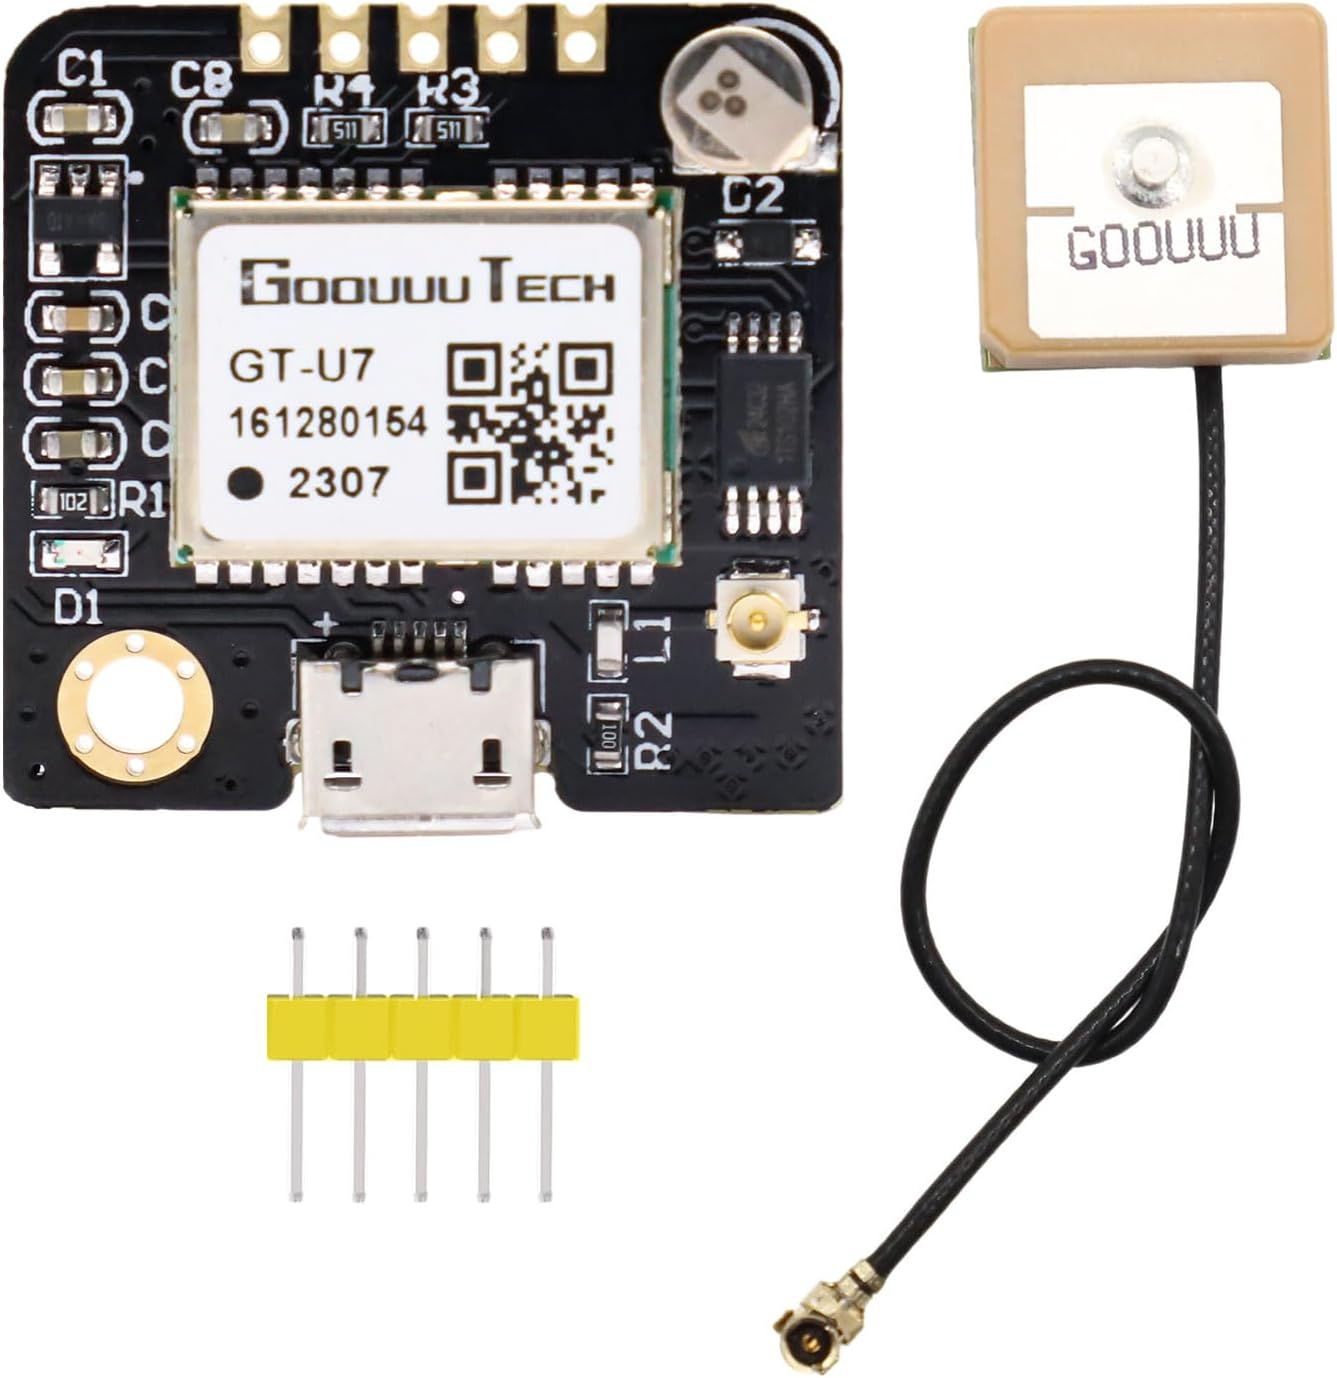
\includegraphics[width=0.5\textwidth]{material/gps-module.jpg}
            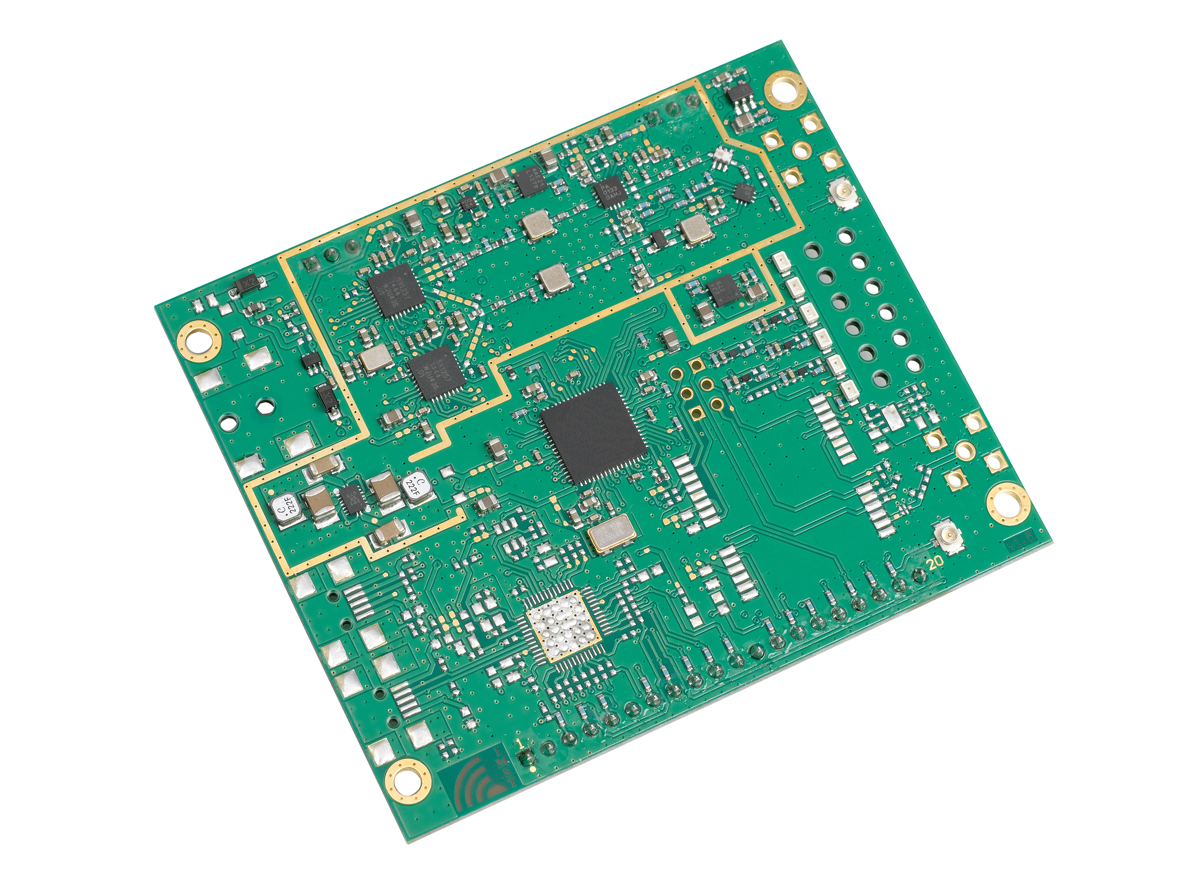
\includegraphics[width=0.5\textwidth]{material/ic880a-spi.png}
        \end{center}
    \end{column}
\end{columns}
\begin{itemize}
\item Basierend auf einem \alert{Raspberry Pi} (3, 4, 5) und \href{https://github.com/lorabasics/basicstation?tab=readme-ov-file}{LoRa Basics™ Station}.
\item LoRa-Konzentrator: \alert{iC880A-SPI – LoRaWAN-Konzentrator 868\,MHz mit 8 Kanälen}.
\item Präzises Zeitmanagement: \alert{APKLVSR GT-U7 GPS-Empfänger}.
\end{itemize}
\end{frame}
